\documentclass{article}
\usepackage[margin=1in]{geometry}
\usepackage[utf8]{vietnam}
\usepackage{hyperref}
\usepackage{cite}
\usepackage{amsmath,amssymb,amsfonts}
\usepackage{algorithmic}
\usepackage{graphicx}
\usepackage{textcomp}
\usepackage{array}
\usepackage[table]{xcolor}
\usepackage{multirow}
\usepackage{multicol}
\usepackage{float}
\usepackage[vietnamese]{babel}
\usepackage{titling}


\pretitle{\begin{center}\fontsize{40pt}{40pt}\bfseries} % Chỉnh kích thước và định dạng cho phần tiêu đề
\posttitle{\end{center}} % Kết thúc định dạng cho phần tiêu đề

\setlength{\droptitle}{-4em} % Điều chỉnh khoảng cách giữa tiêu đề và nội dung

\begin{document}

\title{Phân tích, dự đoán giá chứng khoản bằng mô hình thống kê}
\author{
  \begin{tabular}{l}
    \textbf{Trần Thị Mỹ Xoan - 21522815 } \\
    \textbf{Lê Anh Tuấn Dũng - 21521974} \\
    \textbf{Lê Thị Ánh Hồng - 21520245} \\
    \textbf{Nguyễn Thị Mai Liên - 21522283} \\
    \textbf{Đỗ Sĩ Đạt - 21521932}
  \end{tabular}
}




\maketitle


\textbf{Tóm tắt nội dung:}
Khi thực hiện đầu tư vào các cổ phiếu chứng khoán, việc sử dụng các mô hình dự đoán giá cổ phiếu trước khi thực hiện một giao dịch đầu tư có thể giúp cho ta có các quyết định đúng đắn hơn khi ra quyết định thực hiện 1 giao dịch. Bài báo này trình bày phương pháp dự đoán giá cổ phiếu của ba công ty lớn Samsung, LG và Sony. Chúng tôi sẽ thực hiện dự đoán bằng cách sử dụng các thuật toán thống kê: ARIMA, Linear Regression, VARMA. Bộ dữ liệu được sử dụng lấy từ ngày 1/3/2019 đến ngày 1/6/2024. Sau khi thực hiện dự đoán thì ta sẽ thực hiện sử dụng các độ đo MAPE, MSE, RMSE để đánh giá các mô hình. Cuối cùng, sử dụng các mô hình để thực hiện dự đoán giá chứng khoán cho 30, 60 và 90 ngày tiếp theo.


\vspace{1em} % Thêm khoảng cách


\textbf{Từ khoá:} ARIMA, Linear Regression, VARMA. Phân tích, dự đoán giá chứng khoán.

\begin{multicols}{2}

\section{GIỚI THIỆU}
Dự đoán giá cổ phiếu là một vấn đề quan trọng trong lĩnh vực đầu tư tài chính. Việc dự đoán chính xác giá cổ phiếu có thể giúp các nhà đầu tư đưa ra quyết định đầu tư sáng suốt và giảm thiểu rủi ro. Có nhiều phương pháp khác nhau để dự đoán giá cổ phiếu, bao gồm phân tích kỹ thuật, phân tích cơ bản và học máy. Samsung, LG, SONY là những công ty hàng đầu trong ngành công nghệ, giá cổ phiếu của 3 công ty đóng vai trò là chỉ số quan trọng về động lực thị trường, khiến việc phân tích của họ trở nên cần thiết đối với các nhà đầu tư. 

Báo cáo này nhằm mục đích phân tích, dự đoán giá cổ phiếu của các công ty có ảnh hưởng bằng cách sử dụng 3 thuật toán ARIMA, Linear Regression, VARMA để đưa ra dự đoán cho giá cổ phiếu. Nhờ đó các nhà đầu tư có thể lựa chọn chính xác hạng mục đầu tư vào giá cổ phiếu. 

Bằng cách tận dụng những phương pháp này, chúng tôi mong muốn cung cấp hướng dẫn có giá trị cho các nhà dầu tư trong việc định hướng bối cảnh năng động của lĩnh vực công nghệ. 


\section{NGHIÊN CỨU LIÊN QUAN}


[1] Mô hình VARMA thường được sử dụng để dự báo dữ liệu chuỗi thời gian đa biến. Mô hình VARMA là sự mở rộng của mô hình ARMA trong chuỗi thời gian đơn biến (Lütkepohl, 2005; Wei, 1990) và được sử dụng với điều kiện rằng dữ liệu phải ổn định theo thời gian (Lütkepohl, 2005). Mô hình VARMA (p,q) là sự kết hợp của mô hình VAR (p) và mô hình vector trung bình động (q) (VMA (q)). Bài báo này xác định 4 mô hình VARMA (p,q) lần lượt là (1,1), (2, 1), (3, 1), (4, 1), Việc lựa chọn mô hình tốt nhất được thực hiện bằng cách sử dụng một số tiêu chí thông tin (AICC, HQC, AIC, và SBC). Các giá trị nhỏ nhất của những tiêu chí này cho biết mô hình tốt nhất. Mô hình phù hợp nhất được chọn là VARMA(2, 1). Kết quả dự báo cho thấy sai số chuẩn tăng lên theo thời gian; sai số chuẩn trong tháng đầu tiên tương đối nhỏ so với dự đoán trung bình, nhưng tăng lên theo thời gian đến dự báo cho 12 tháng tiếp theo. Điều này cho thấy mô hình là hợp lý khi dự báo cho các khoảng thời gian ngắn, nhưng kết quả không ổn định (do sai số chuẩn cao hơn) khi dự báo cho các khoảng thời gian dài.

\section{PHƯƠNG PHÁP}




\subsection{THUẬT TOÁN VARMA}
Mô hình VARMA thường được sử dụng để dự báo dữ liệu chuỗi thời gian đa biến . Mô hình VARMA là một mở rộng của mô hình ARMA trong chuỗi thời gian đơn biến (Lutkepohl, 2005; Wei, 1990) và được sử dụng với điều kiện dữ liệu phải là dừng theo thời gian (Lutkepohl, 2005). Mô hình VARMA (p,q) là sự kết hợp của mô hình VAR (p) và mô hình trung bình trượt vector (q) (VMA (q)).\\
 
    • Công thức:
    \begin{equation}
        \mathbf{y}_t = \mathbf{c} + \sum_{i=1}^{p} \mathbf{\Phi}_i \mathbf{y}_{t-i} + \sum_{j=1}^{q} \mathbf{\Theta}_j \boldsymbol{\epsilon}_{t-j} + \boldsymbol{\epsilon}_t
    \end{equation}  
Trong đó:  
    \begin{itemize}
      \item \( \mathbf{y}_t \) là vector của các biến tại thời điểm \( t \).
      \item \( \mathbf{c} \) là một vector hằng số.
      \item \( \mathbf{\Phi}_i \) là ma trận hệ số của chuỗi thời gian ( độ trễ, lag) \( i \) của mô hình AR.
      \item \( \mathbf{\Theta}_j \) là ma trận hệ số của chuỗi thời gian ( độ trễ, lag) \( j \) của mô hình MA.
      \item \( \boldsymbol{\epsilon}_t \) là vector của các nhiễu ngẫu nhiên tại thời điểm \( t \).
    \end{itemize} 

\section{THỰC NGHIỆM}

\subsection{MÔ HÌNH DỰ ĐOÁN }
\subsubsection{ARIMA}
  
\subsubsection{LINEAR REGRESSION}

\subsubsection{VARMA}
\begin{figure}[H]
    \centering
    \begin{minipage}{0.15\textwidth}
    \centering
    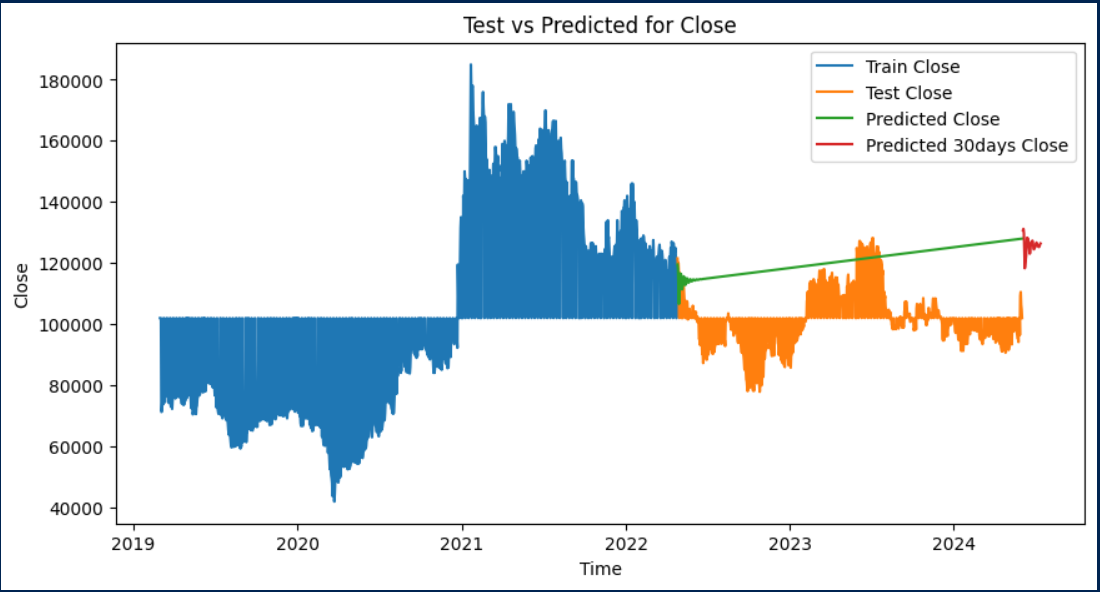
\includegraphics[width=1\textwidth]{Image/VARMA/LG/6_4/30.png}
   
    \label{fig:1}
    \end{minipage}%
    \begin{minipage}{0.15\textwidth}
    \centering
    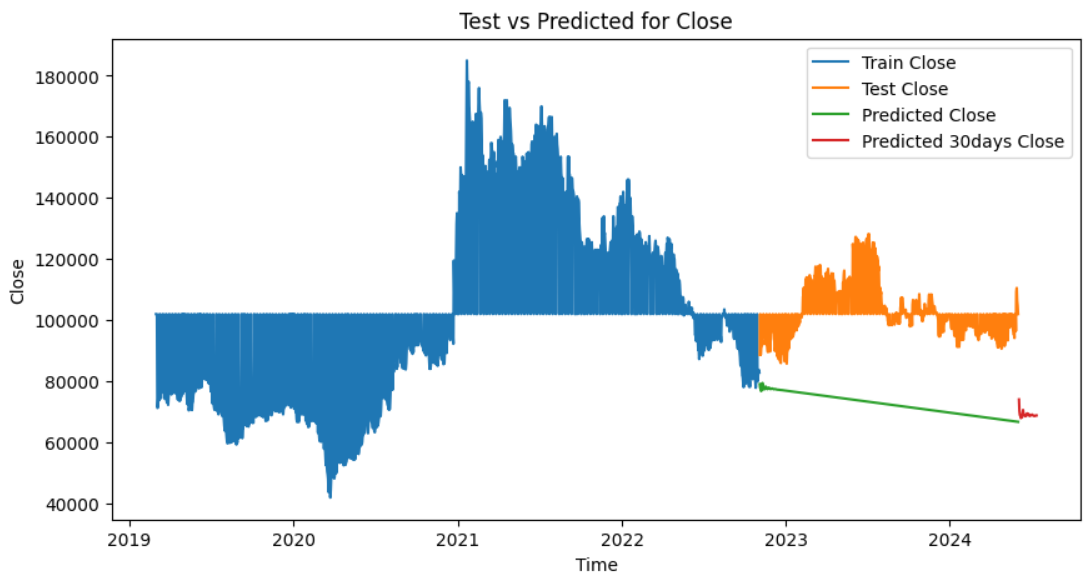
\includegraphics[width=1\textwidth]{Image/VARMA/LG/7_3/30.png}
  
    \label{fig:2}
    \end{minipage}%
    \begin{minipage}{0.15\textwidth}
    \centering
    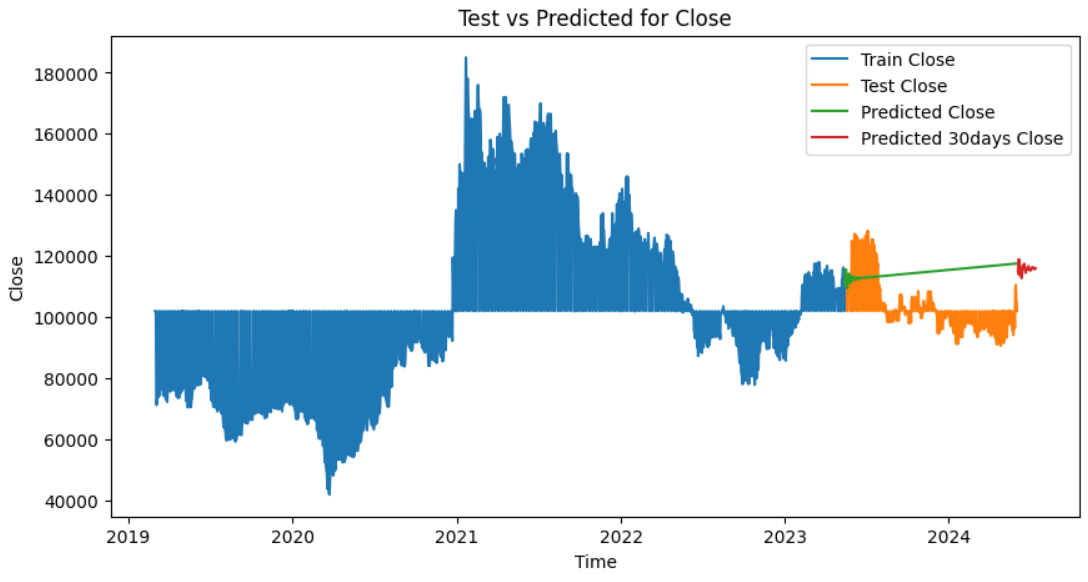
\includegraphics[width=1\textwidth]{Image/VARMA/LG/8_2/30.png}

    \label{fig:3}
    \end{minipage}
    \caption{LG 30 DAYS  6:4, 7:3, 8:2 }
\end{figure}

\begin{figure}[H]
    \centering
    \begin{minipage}{0.15\textwidth}
    \centering
    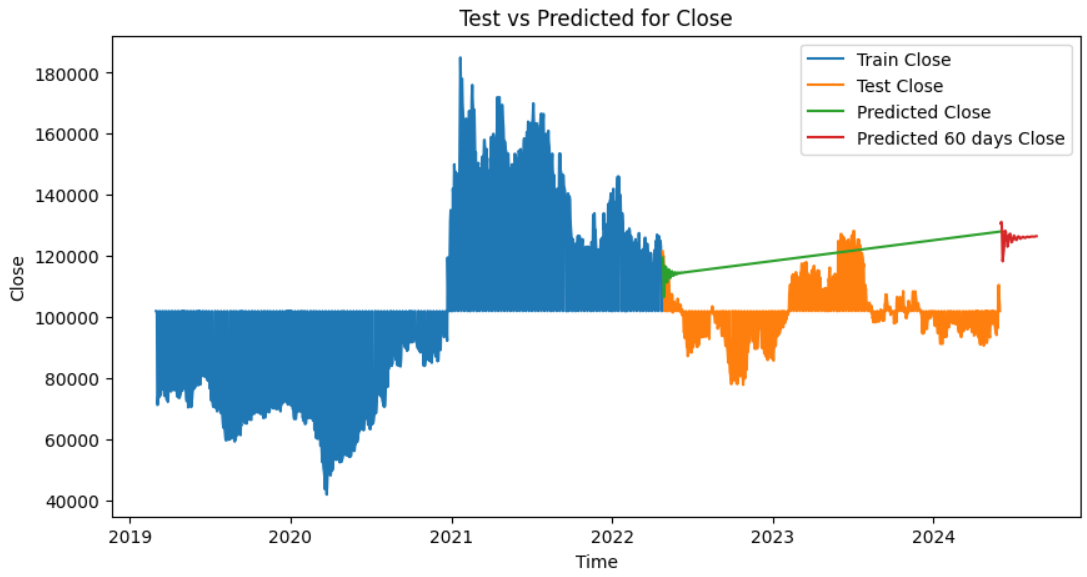
\includegraphics[width=1\textwidth]{Image/VARMA/LG/6_4/60.png}
   
    \label{fig:1}
    \end{minipage}%
    \begin{minipage}{0.15\textwidth}
    \centering
    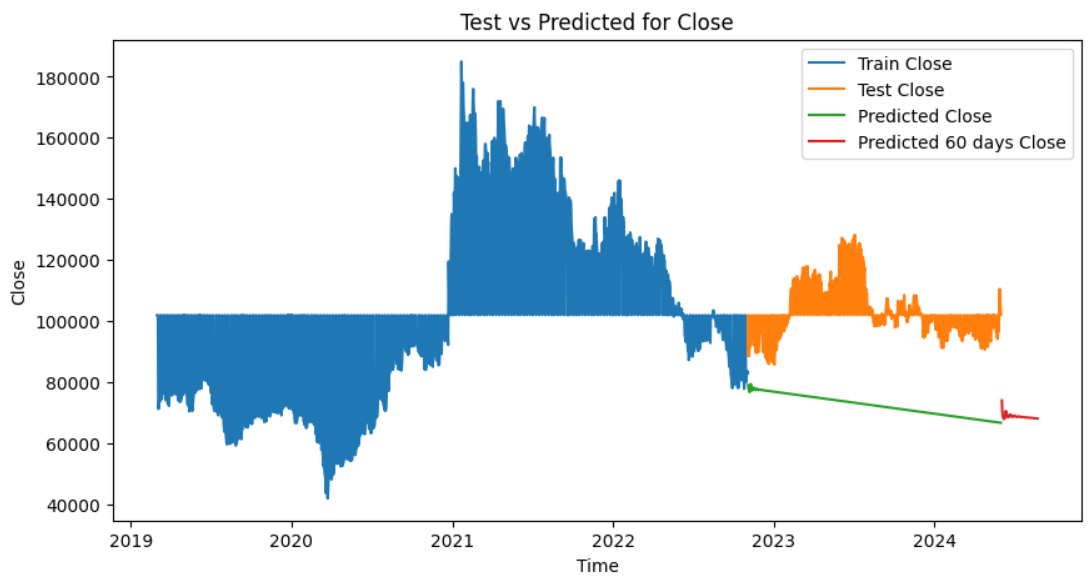
\includegraphics[width=1\textwidth]{Image/VARMA/LG/7_3/60.png}
  
    \label{fig:2}
    \end{minipage}%
    \begin{minipage}{0.15\textwidth}
    \centering
    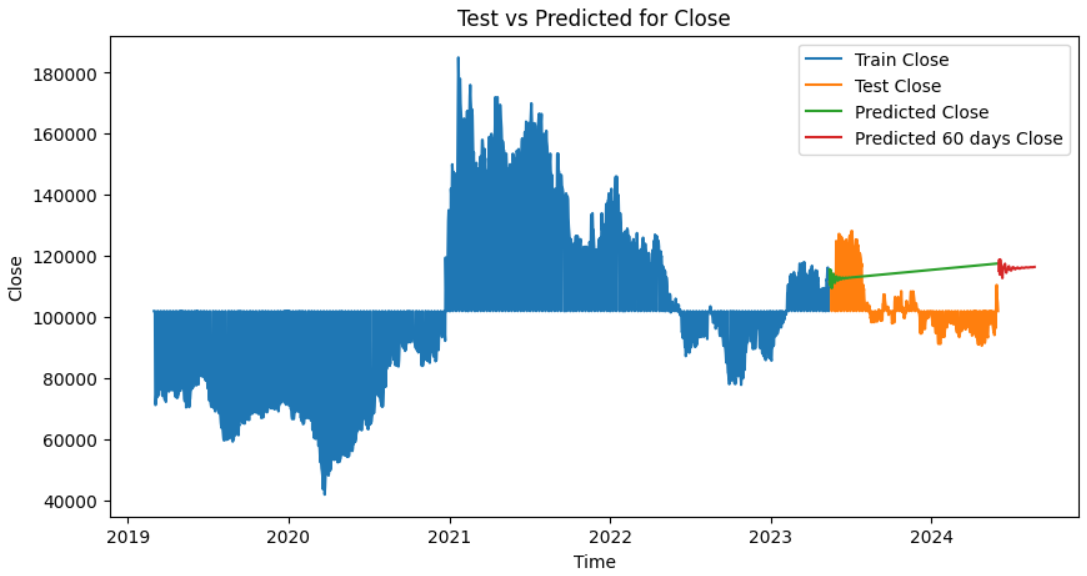
\includegraphics[width=1\textwidth]{Image/VARMA/LG/8_2/60.png}

    \label{fig:3}
    \end{minipage}
    \caption{LG 60 DAYS  6:4, 7:3, 8:2 }
\end{figure}

\begin{figure}[H]
    \centering
    \begin{minipage}{0.15\textwidth}
    \centering
    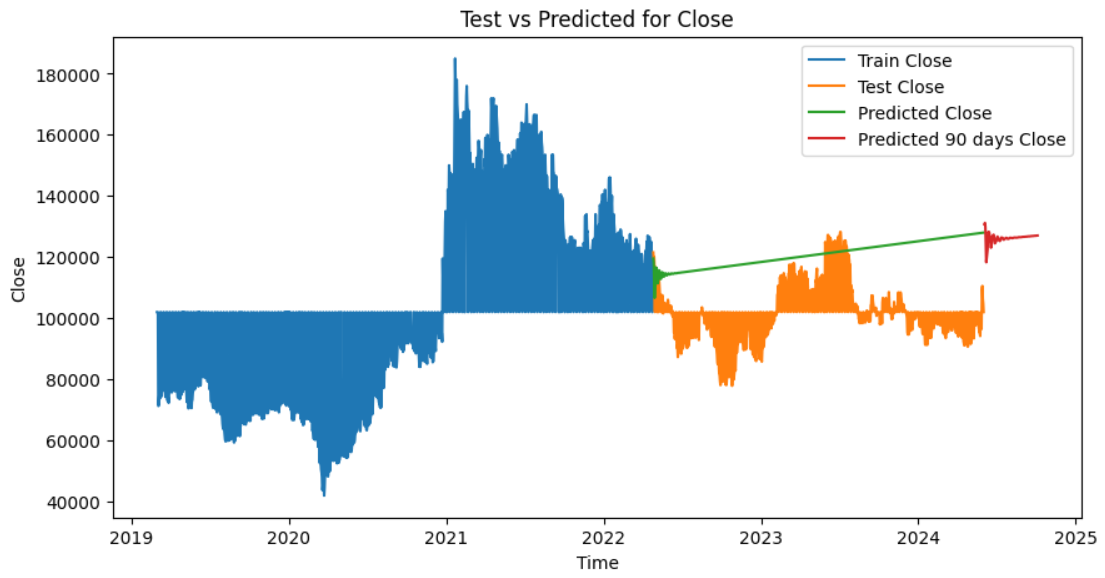
\includegraphics[width=1\textwidth]{Image/VARMA/LG/6_4/90.png}
   
    \label{fig:1}
    \end{minipage}%
    \begin{minipage}{0.15\textwidth}
    \centering
    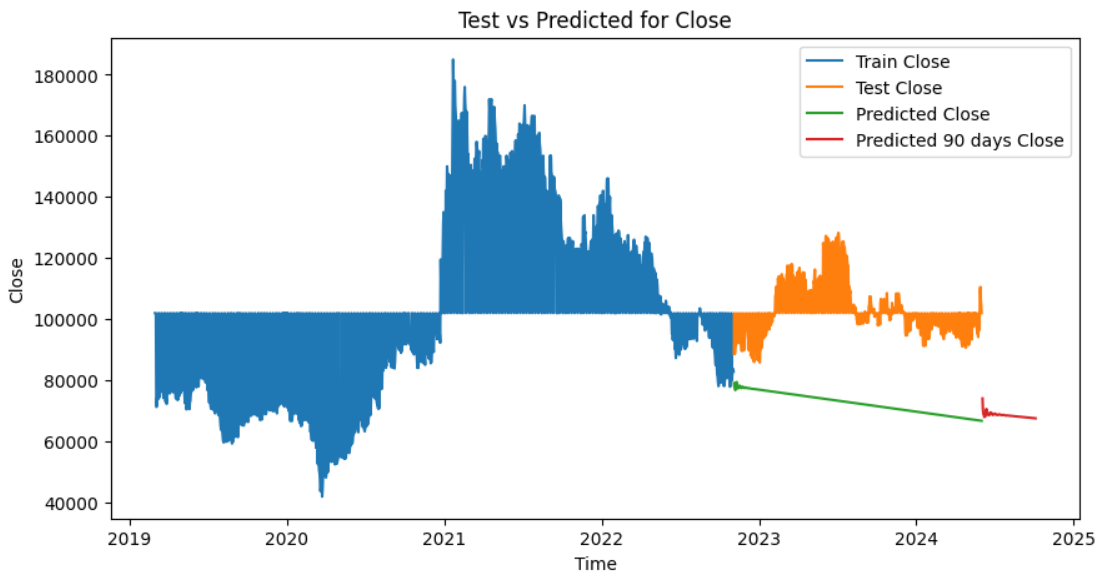
\includegraphics[width=1\textwidth]{Image/VARMA/LG/7_3/90.png}
  
    \label{fig:2}
    \end{minipage}%
    \begin{minipage}{0.15\textwidth}
    \centering
    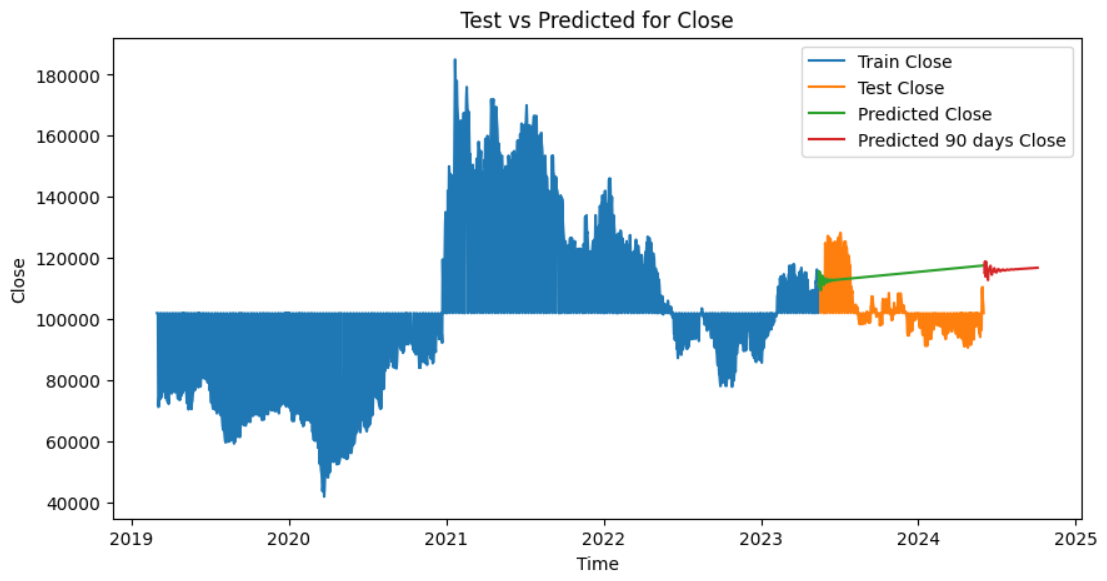
\includegraphics[width=1\textwidth]{Image/VARMA/LG/8_2/90.png}

    \label{fig:3}
    \end{minipage}
    \caption{LG 90 DAYS  6:4, 7:3, 8:2 }
\end{figure}

\begin{figure}[H]
    \centering
    \begin{minipage}{0.15\textwidth}
    \centering
    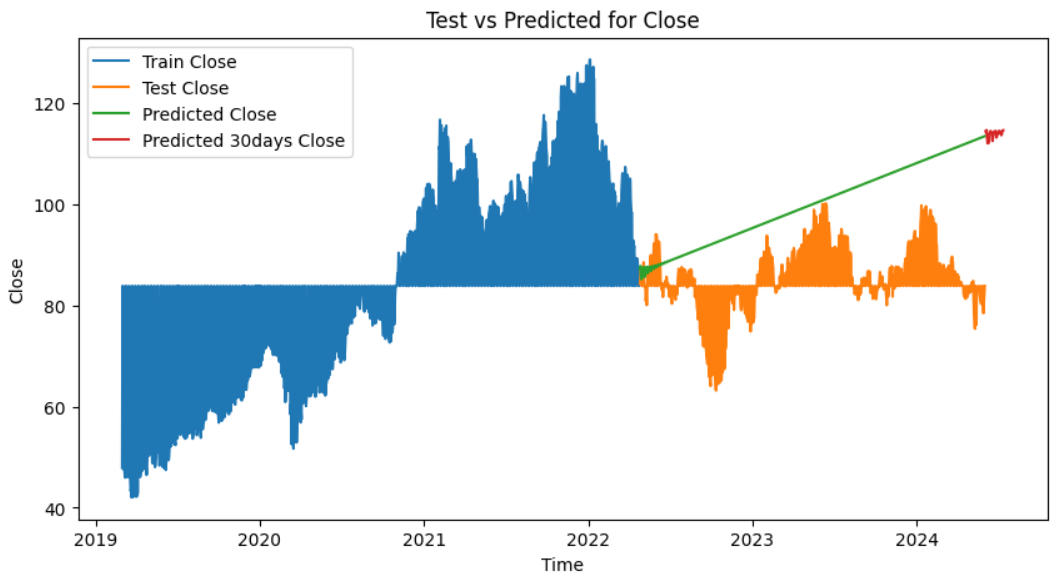
\includegraphics[width=1\textwidth]{Image/VARMA/SONY/6_4/30.png}
   
    \label{fig:1}
    \end{minipage}%
    \begin{minipage}{0.15\textwidth}
    \centering
    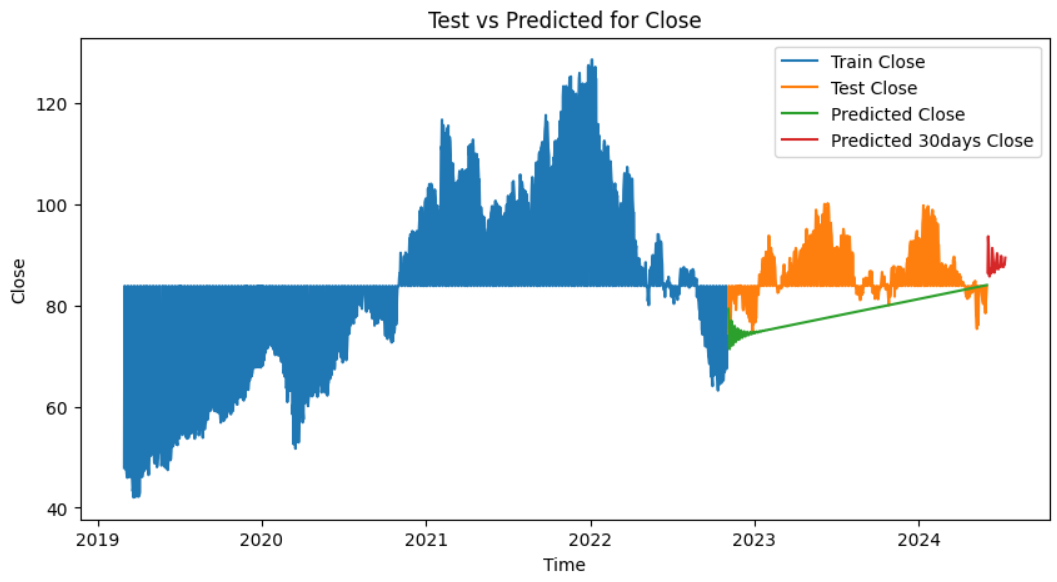
\includegraphics[width=1\textwidth]{Image/VARMA/SONY/7_3/30.png}
  
    \label{fig:2}
    \end{minipage}%
    \begin{minipage}{0.15\textwidth}
    \centering
    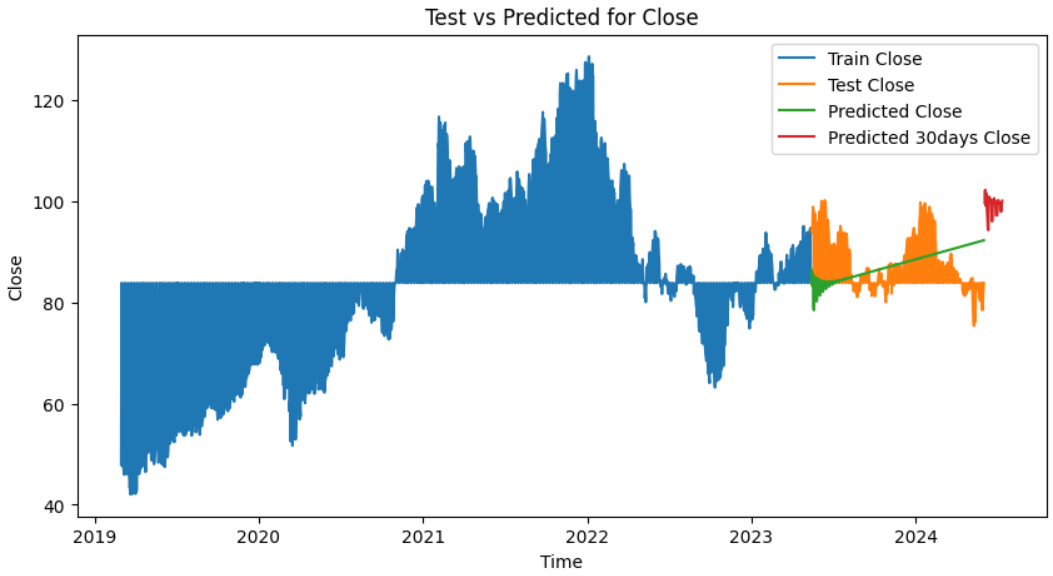
\includegraphics[width=1\textwidth]{Image/VARMA/SONY/8_2/30.png}

    \label{fig:3}
    \end{minipage}
    \caption{SONY 30 DAYS  6:4, 7:3, 8:2 }
\end{figure}

\begin{figure}[H]
    \centering
    \begin{minipage}{0.15\textwidth}
    \centering
    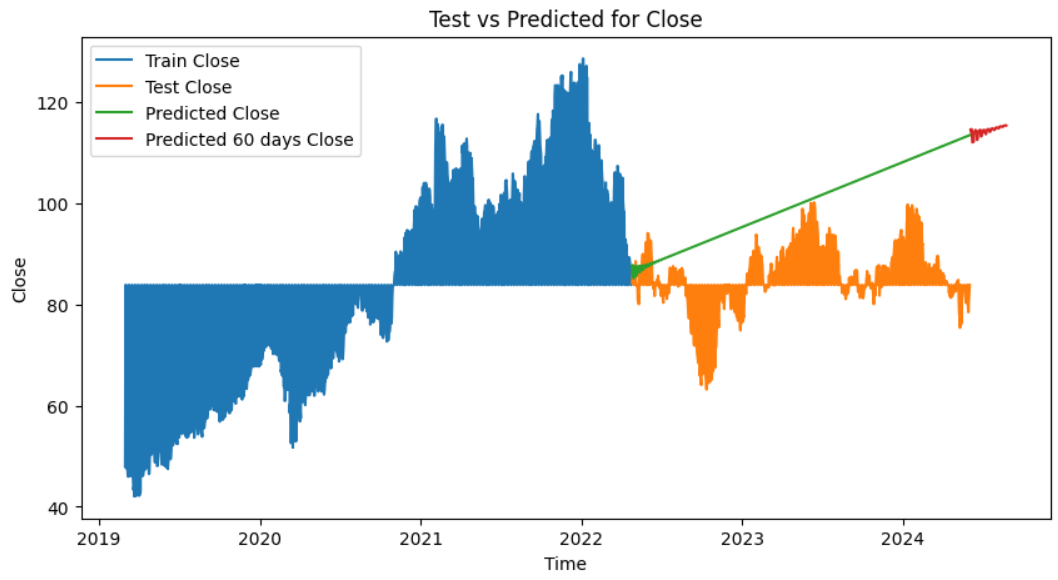
\includegraphics[width=1\textwidth]{Image/VARMA/SONY/6_4/60.png}
   
    \label{fig:1}
    \end{minipage}%
    \begin{minipage}{0.15\textwidth}
    \centering
    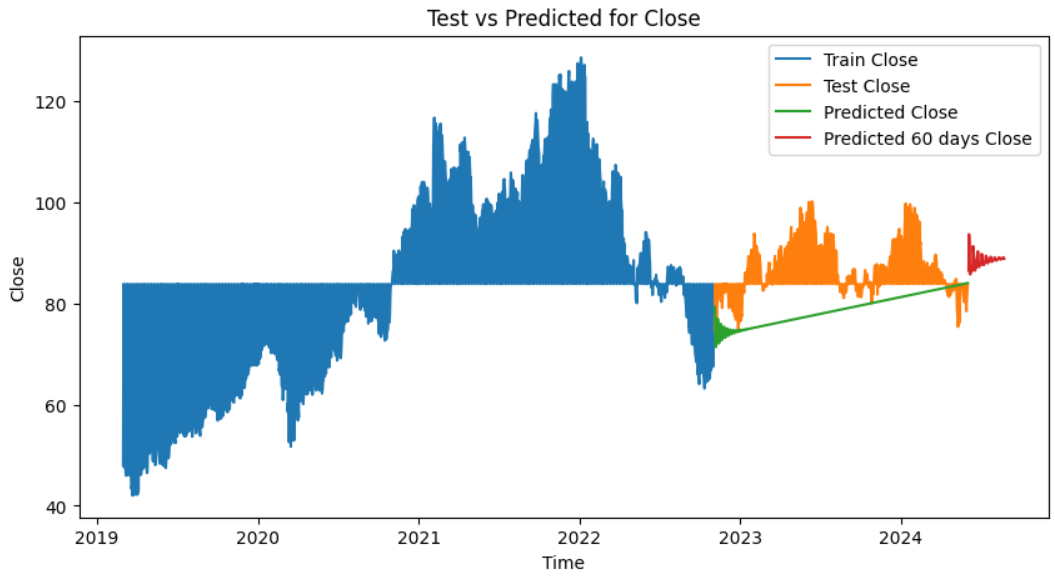
\includegraphics[width=1\textwidth]{Image/VARMA/SONY/7_3/60.png}
  
    \label{fig:2}
    \end{minipage}%
    \begin{minipage}{0.15\textwidth}
    \centering
    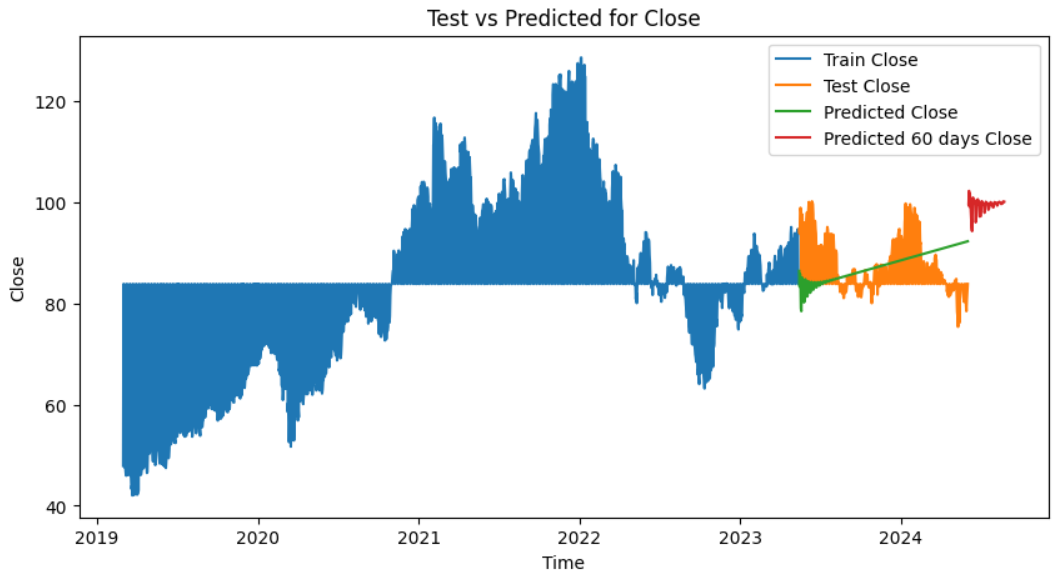
\includegraphics[width=1\textwidth]{Image/VARMA/SONY/8_2/60.png}

    \label{fig:3}
    \end{minipage}
    \caption{SONY 60 DAYS  6:4, 7:3, 8:2 }
\end{figure}

\begin{figure}[H]
    \centering
    \begin{minipage}{0.15\textwidth}
    \centering
    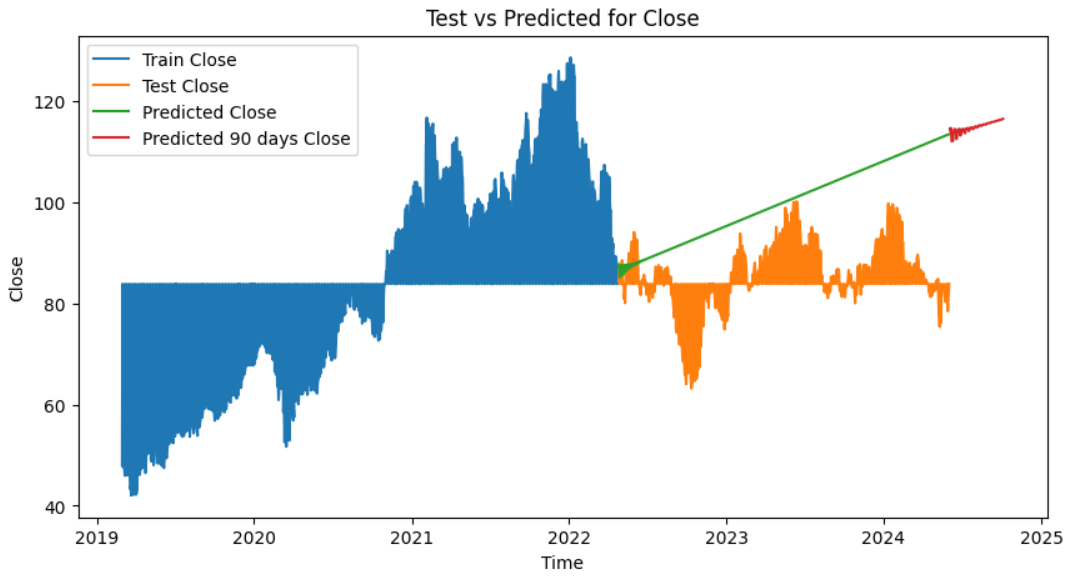
\includegraphics[width=1\textwidth]{Image/VARMA/SONY/6_4/90.png}
   
    \label{fig:1}
    \end{minipage}%
    \begin{minipage}{0.15\textwidth}
    \centering
    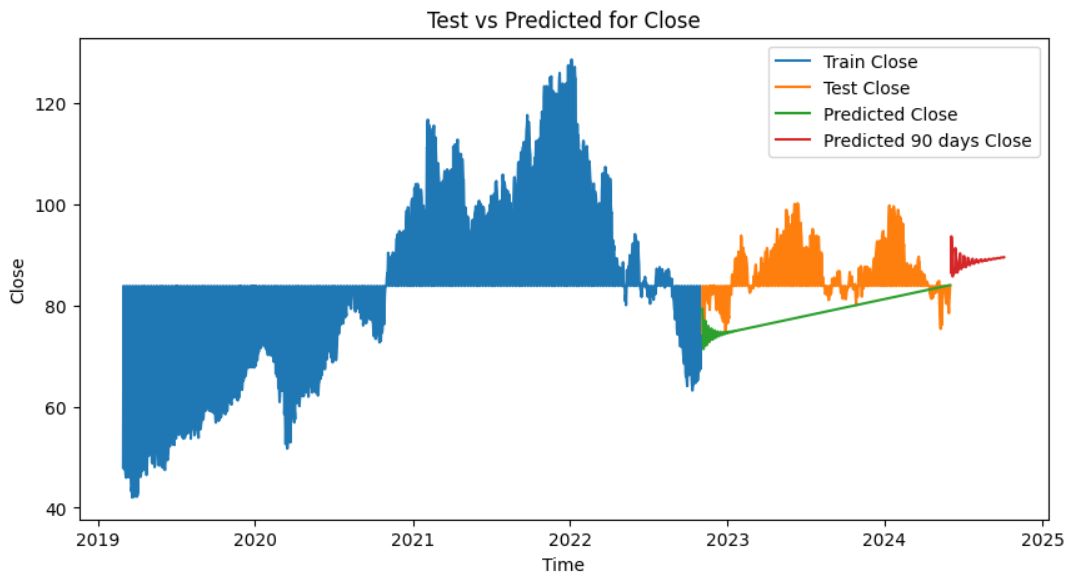
\includegraphics[width=1\textwidth]{Image/VARMA/SONY/7_3/90.png}
  
    \label{fig:2}
    \end{minipage}%
    \begin{minipage}{0.15\textwidth}
    \centering
    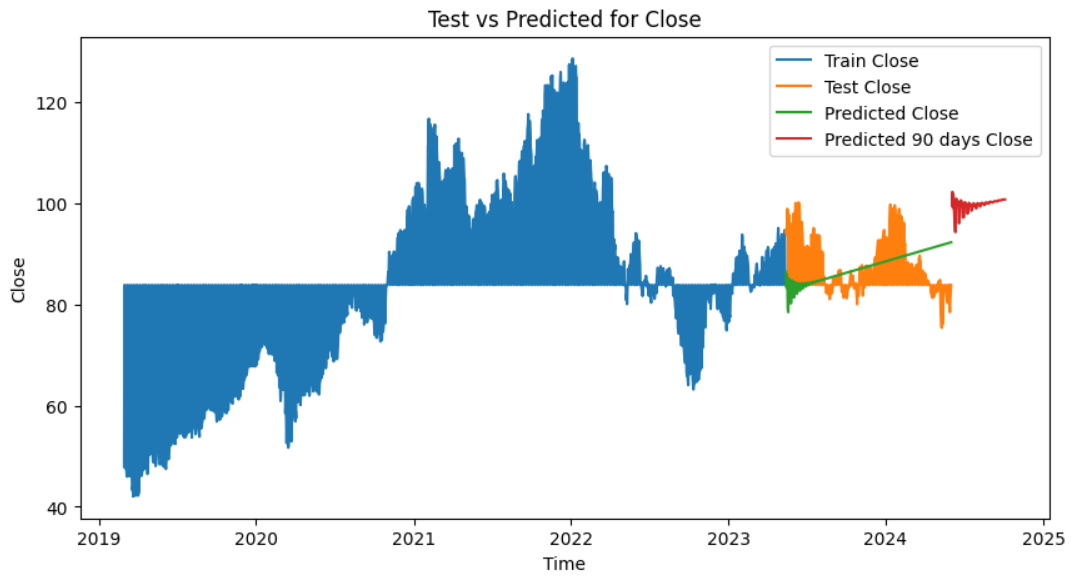
\includegraphics[width=1\textwidth]{Image/VARMA/SONY/8_2/90.png}

    \label{fig:3}
    \end{minipage}
    \caption{SONY 90 DAYS  6:4, 7:3, 8:2 }
\end{figure}

\begin{figure}[H]
    \centering
    \begin{minipage}{0.15\textwidth}
    \centering
    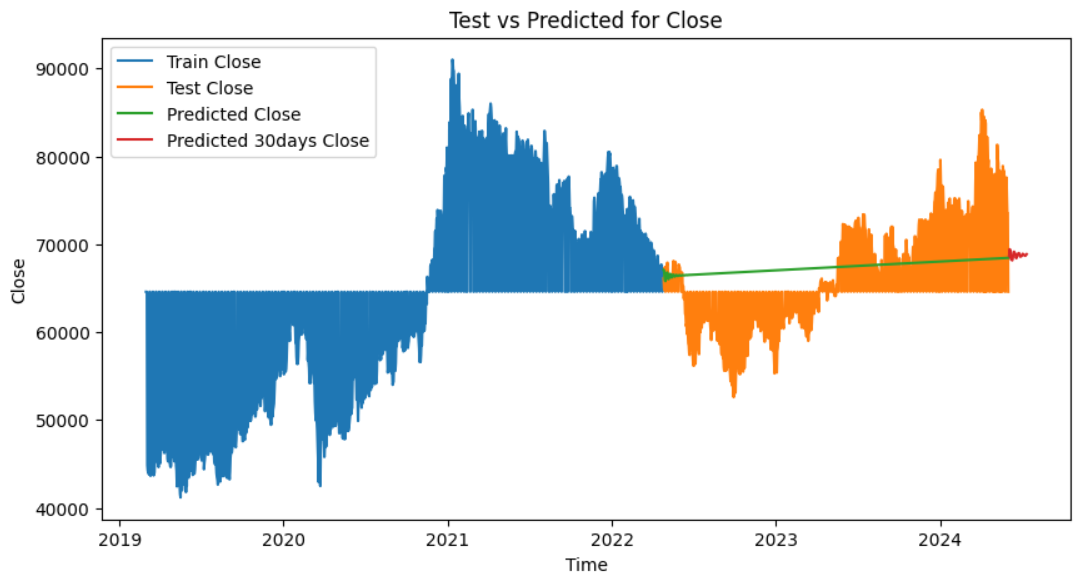
\includegraphics[width=1\textwidth]{Image/VARMA/SAMSUNG/6_4/30.png}
   
    \label{fig:1}
    \end{minipage}%
    \begin{minipage}{0.15\textwidth}
    \centering
    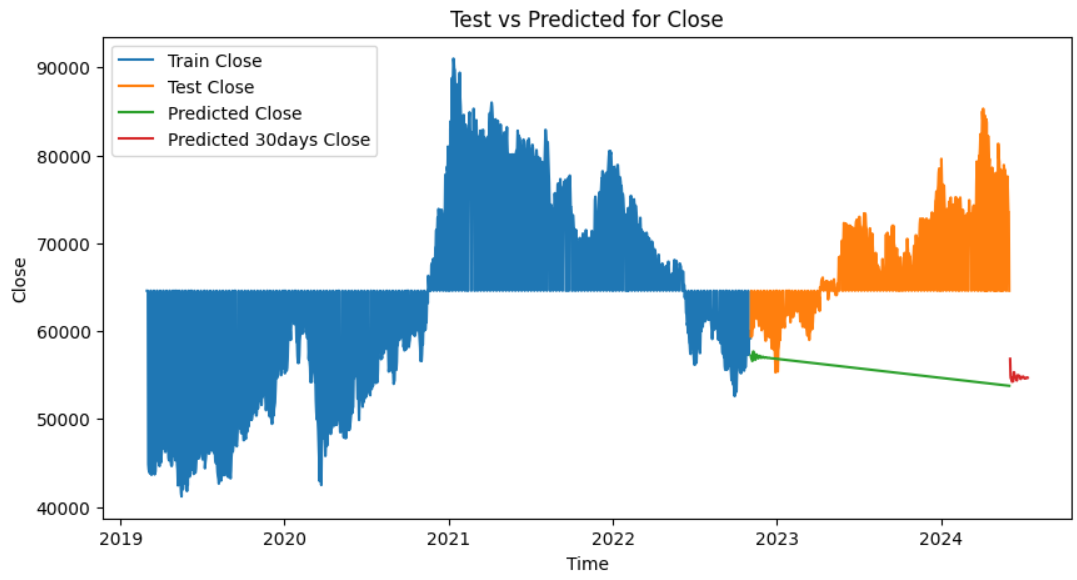
\includegraphics[width=1\textwidth]{Image/VARMA/SAMSUNG/7_3/30.png}
  
    \label{fig:2}
    \end{minipage}%
    \begin{minipage}{0.15\textwidth}
    \centering
    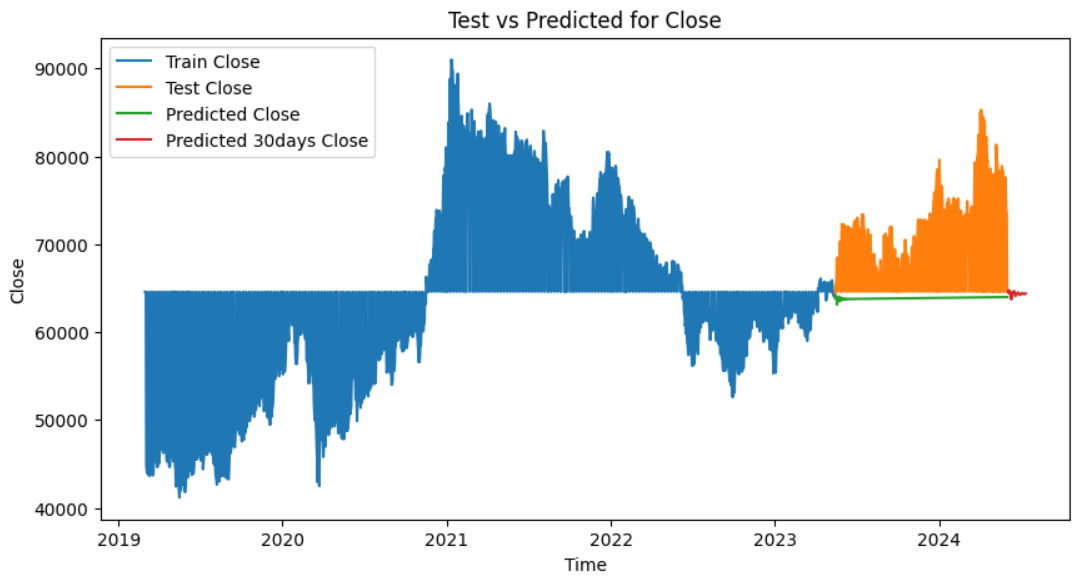
\includegraphics[width=1\textwidth]{Image/VARMA/SAMSUNG/8_2/30.png}

    \label{fig:3}
    \end{minipage}
    \caption{SAMSUNG 30 DAYS  6:4, 7:3, 8:2 }
\end{figure}

\begin{figure}[H]
    \centering
    \begin{minipage}{0.15\textwidth}
    \centering
    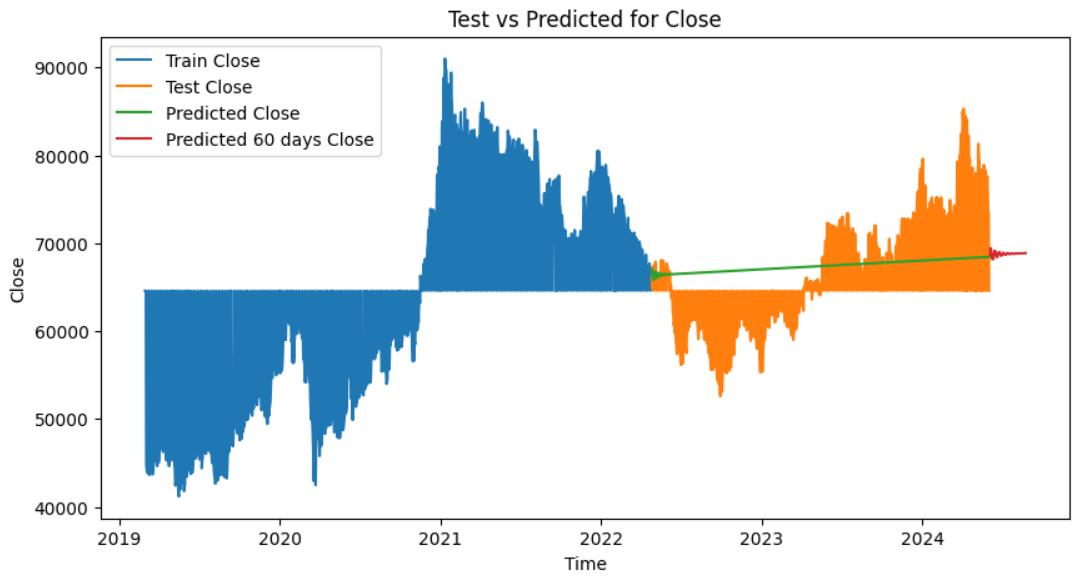
\includegraphics[width=1\textwidth]{Image/VARMA/SAMSUNG/6_4/60.png}
   
    \label{fig:1}
    \end{minipage}%
    \begin{minipage}{0.15\textwidth}
    \centering
    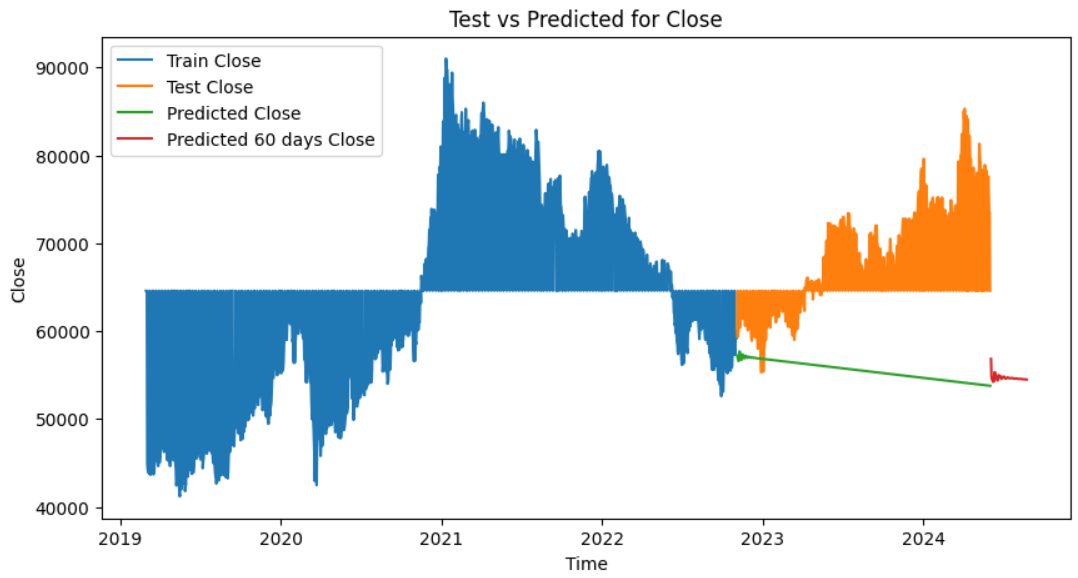
\includegraphics[width=1\textwidth]{Image/VARMA/SAMSUNG/7_3/60.png}
  
    \label{fig:2}
    \end{minipage}%
    \begin{minipage}{0.15\textwidth}
    \centering
    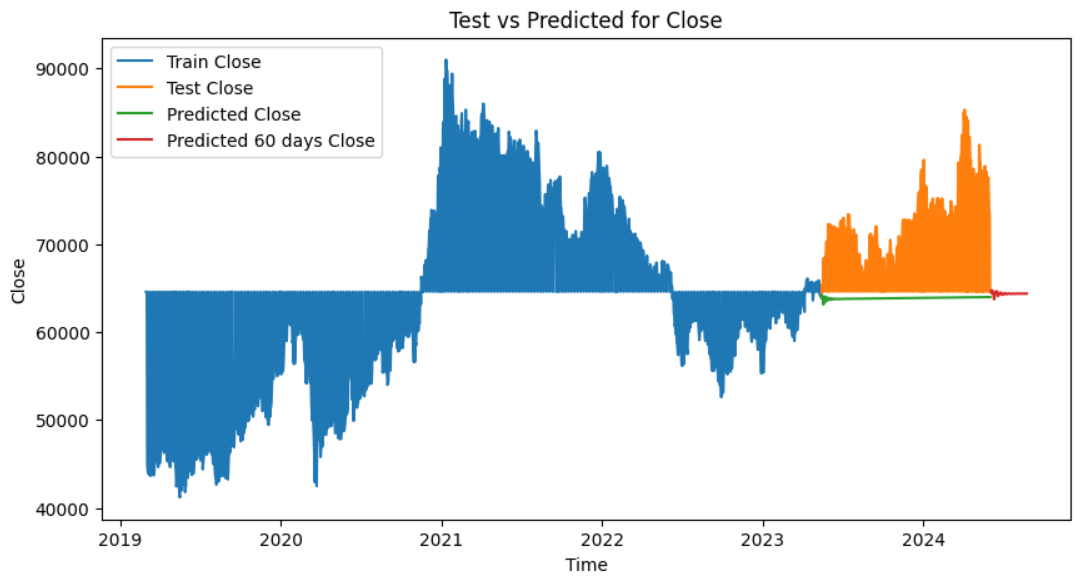
\includegraphics[width=1\textwidth]{Image/VARMA/SAMSUNG/8_2/60.png}

    \label{fig:3}
    \end{minipage}
    \caption{SAMSUNG 60 DAYS  6:4, 7:3, 8:2 }
\end{figure}

\begin{figure}[H]
    \centering
    \begin{minipage}{0.15\textwidth}
    \centering
    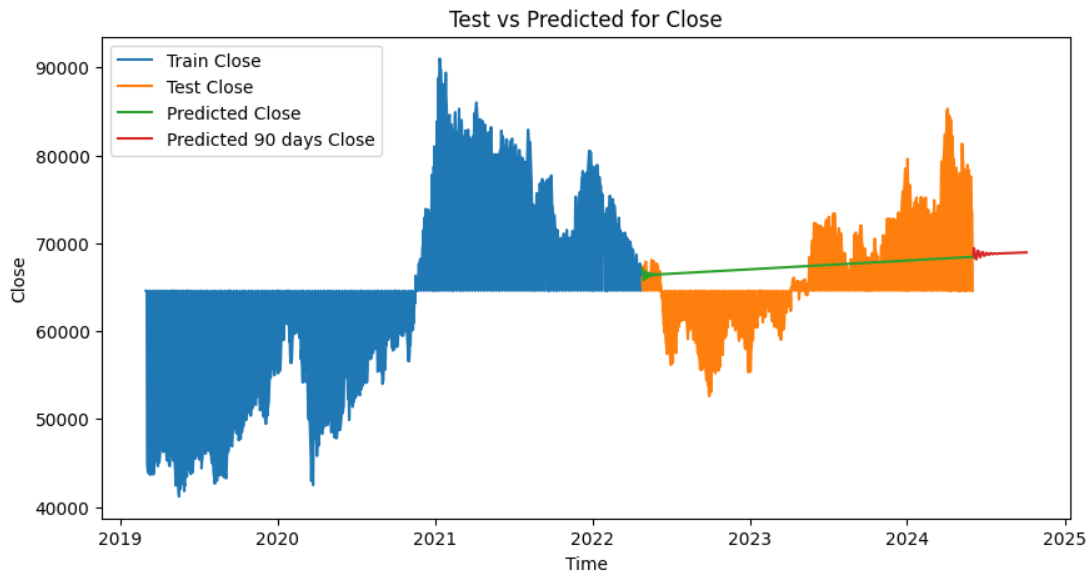
\includegraphics[width=1\textwidth]{Image/VARMA/SAMSUNG/6_4/90.png}
   
    \label{fig:1}
    \end{minipage}%
    \begin{minipage}{0.15\textwidth}
    \centering
    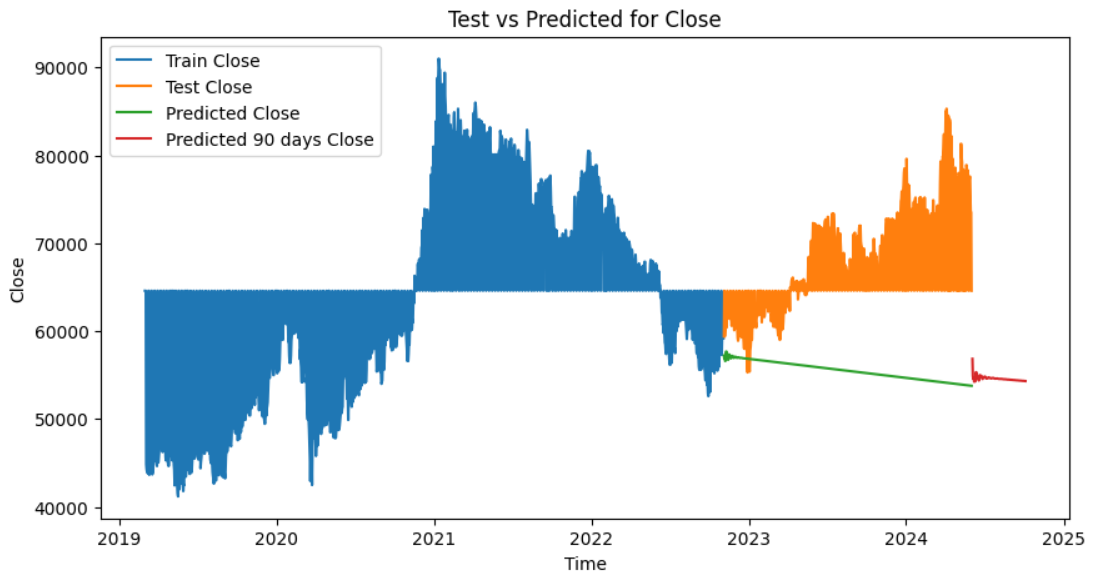
\includegraphics[width=1\textwidth]{Image/VARMA/SAMSUNG/7_3/90.png}
  
    \label{fig:2}
    \end{minipage}%
    \begin{minipage}{0.15\textwidth}
    \centering
    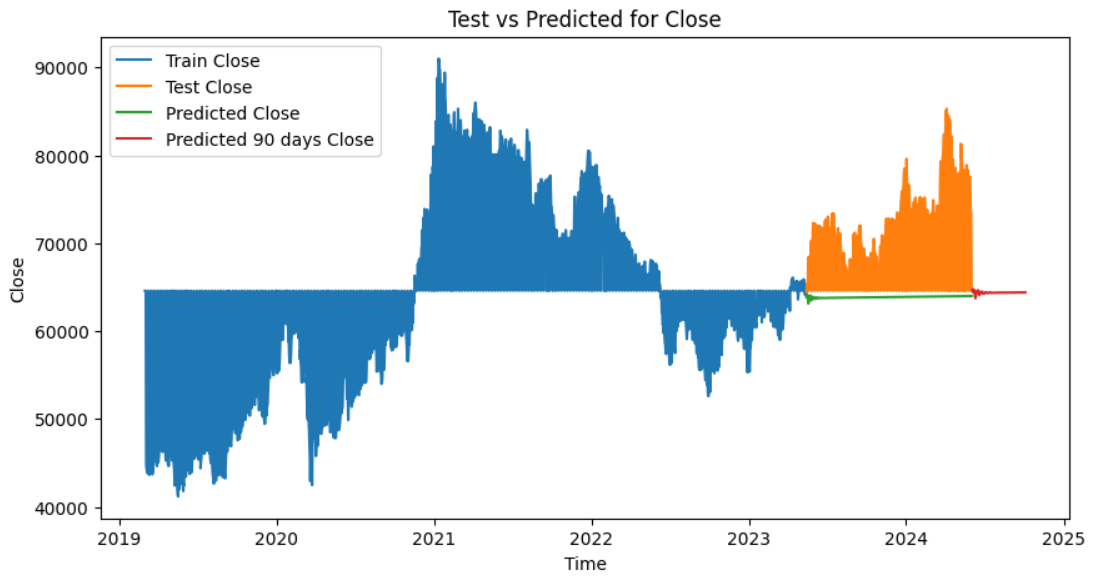
\includegraphics[width=1\textwidth]{Image/VARMA/SAMSUNG/8_2/90.png}

    \label{fig:3}
    \end{minipage}
    \caption{SAMSUNG 90 DAYS  6:4, 7:3, 8:2 }
\end{figure}

\section{TÀI LIỆU THAM KHẢO}

 
[1]: Warsono, Edwin Russel, Wamiliana*, Widiarti, Mustofa Usman, "Modeling and Forecasting by the Vector Autoregressive Moving Average Model for Export of Coal and Oil Data (Case Study from Indonesia over the Years 2002-2017)". International Journal of Energy Economics and Policy, 2019

\bibliographystyle{plain}

\end{multicols}
\end{document}

